\documentclass{article}

\usepackage[utf8]{inputenc}
\usepackage[spanish]{babel}
\usepackage[a4paper,top=2cm,bottom=2cm,left=3cm,right=3cm,marginparwidth=1.75cm]{geometry}
\usepackage{amsmath}
\usepackage{graphicx}
\graphicspath{{imagenes/}}
\usepackage{float}
\usepackage{caption}
\usepackage[colorlinks=true, allcolors=blue]{hyperref}

\title{\textbf{%
    Universidad Nacional de San Agustín \\
    Maestría en Ciencias de la Computación \\
    \large Análisis del Problema del Agente Viajero}}
\author{Abel E. Borit Guitton, Luis A. Borit Guitton, Betzy J. Yarín Ramírez}
% \date{\today}
\date{17 de agosto de 2023}

\begin{document}
\maketitle

\section{INTRODUCCION}
\subsection{Introducción al problema del agente viajero}
El problema del agente viajero (Traveling Salesman Problem, TSP) es un problema de optimización combinatoria (se trata de un problema de optimización que involucra una cantidad finita o numerable de soluciones posibles) en el campo de la teoría de la computación y la investigación de operaciones. 

Se trata de encontrar la ruta más corta posible que permita a un agente visitar un conjunto dado de ciudades y regresar a la ciudad de origen, pasando por cada ciudad exactamente una vez.

\subsection{Introducción a heurísticas}
Cuando un algoritmo usa una heurística, ya no necesita buscar de manera exhaustiva todas las soluciones posibles, y por tanto puede encontrar soluciones aproximadas mas rápido. Una heuristica es un atajo que sacrifica exactitud por rapidez.

\subsection{Introducción a metaheurísticas}
Los metaheurísticos son métodos aproximados diseñados para resolver problemas de optimización combinatoria, en los que los heurísticos clásicos no son efectivos.

\subsection{Introducción de Notación Big-O}
La [2] Notación Big-O es una forma de medir el tiempo lo bien que escala un programa o un algoritmo y el tiempo que tardará en ejecutar. Esta medición nos resultará muy útil para comparar la eficiencia de dos algoritmos, por ejemplo de ordenamiento.

\begin{figure}[H]
\centering
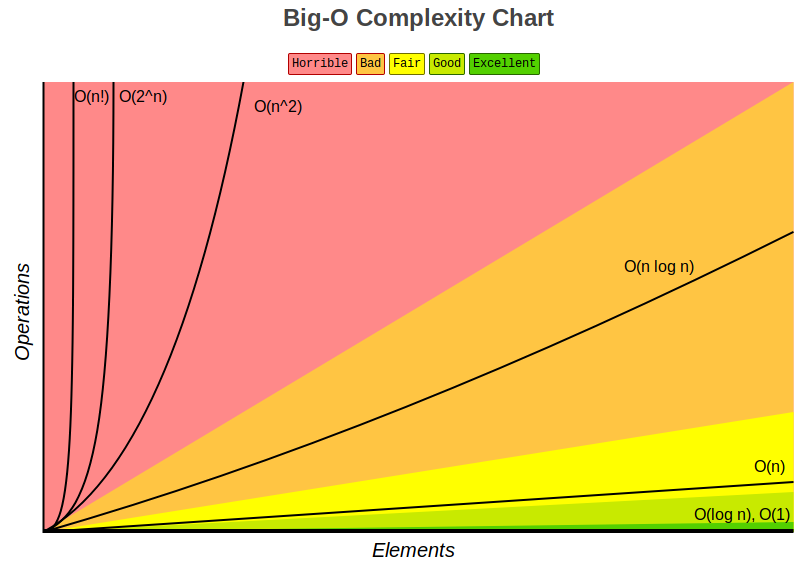
\includegraphics[width=0.6\textwidth]{big-o-complexity-chart.png}
\caption{\label{fig:bigo}Gráfico de complejidad BigO}
\end{figure}

\subsection{Introducción de Matplotlib}
Matplotlib es una librería open source que pertenece a Python en la que se pueden crear visualizaciones animadas, estáticas e interactivas en Python. Se pueden usar gráficas con barras verticales, barras horizontales, líneas, etc.

\begin{figure}[H]
\centering
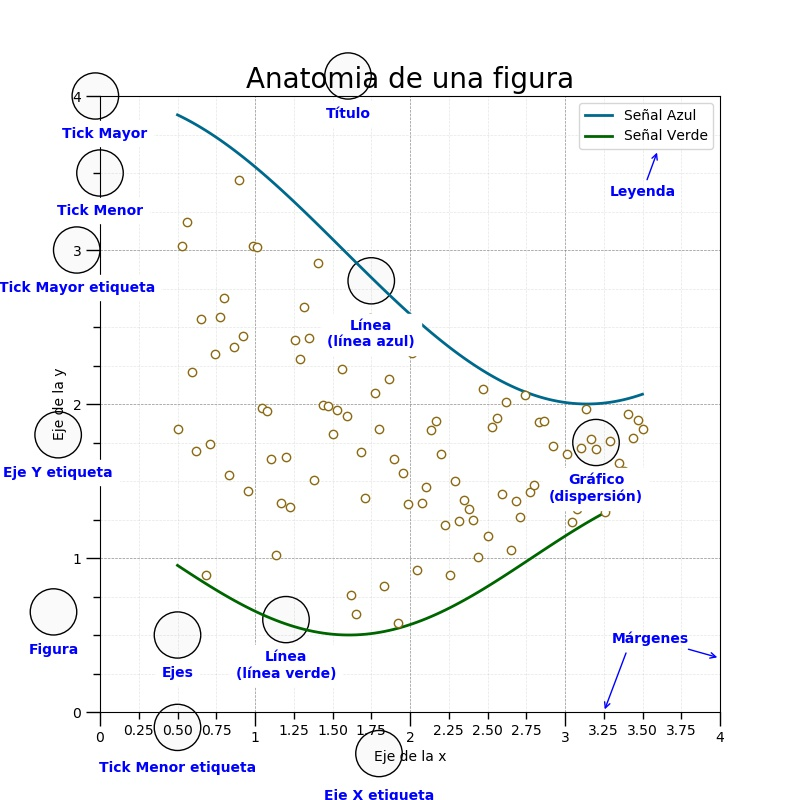
\includegraphics[width=0.6\textwidth]{Anatonia-de-un-grafico-matplotlibjpg.jpg}
\caption{\label{fig:matplotlib}Anatonia de un gráfico matplotlib}
\end{figure}


% *****************************************************************

\section{ALGORITMOS}
\subsection{ALGORITMO DEL ÁRBOL DE EXPANSIÓN MÍNIMA (MINIMUM SPANNING TREE, MST)}
Se construye un árbol de expansión mínima a partir de las ciudades y luego se recorre para formar una ruta. El algoritmo encuentra un subconjunto de aristas que forman un árbol con todos los vértices, donde el peso total de todas las aristas en el árbol es el mínimo posible.

Este algoritmo es ampliamente utilizado en teoría de grafos y optimización combinatoria para encontrar un subconjunto de aristas de un grafo conexo que conecta todos los vértices y tiene un peso total mínimo.

El Algoritmo del Árbol de Expansión Mínima es mejor para grandes cantidades de datos:

    \begin{enumerate}
        \item \textbf{Optimización garantizada:} El MST garantiza una solución óptima para el problema del Agente Viajero si el gráfico (grafo completo con pesos en este caso) cumple con la propiedad del triángulo. Esta propiedad establece que para cualquier conjunto de tres ciudades, el camino más largo entre dos de ellas no es mayor que la suma de los otros dos caminos. Esto asegura que el MST proporcionará una solución cercana a la óptima para TSP.
        
        \item \textbf{Enfoque heurístico:} Aunque no es necesariamente la solución más óptima en todos los casos, el MST se comporta bien en la práctica para muchas instancias de TSP, especialmente para casos con un gran número de ciudades.
        
        \item \textbf{Escalabilidad:} A medida que el número de ciudades aumenta, la diferencia en la eficiencia entre los algoritmos se hace más evidente. El MST es más escalable en términos de tiempo de ejecución.
    \end{enumerate}

% *****************************************************************

\section{IMPLEMENTACION}
En el siguiente enlace \href{https://github.com/abelborit/computer-science-master/tree/main/MCC-01_algorithms-and-data-structures}{Repositorio GitHub} se podrá visualizar toda la implementación realizada. Cuenta con un file system estructurado para cada algoritmo usado, archivos txt de donde se tomarán los datos de entrada para los algoritmos, una carpeta donde está el código usado para realizar gráficas con el Matplotlib como sus gráficas correspondientes y también un archivo README.md propio del proyecto y repositorio.

\section{RESULTADOS}
\subsection{COMPARATIVA DE ALGORITMOS}
    \begin{itemize}
      \item \textbf{TIEMPO PROMEDIO DE EJECUCIÓN (milisegundos):}
        \begin{table}[H]
            \centering
            \begin{tabular}{||c c c c||} 
              \hline
              \textbf{Cantidad de Nodos} & \textbf{Minimum Spanning Tree} & \textbf{XXXXXXXXXX} & \textbf{XXXXXXXXXX} \\ [0.5ex] 
              \hline\hline
              10    &  0.0000   &  0.0000  &  0.0000  \\ [0.5ex]
              20    &  0.0000   &  0.0000  &  0.0000  \\ [0.5ex]
              40    &  0.0000   &  0.0000  &  0.0000  \\ [0.5ex]
              80    &  0.0000   &  0.0000  &  0.0000  \\ [0.5ex]
              160   &  0.0000   &  0.0000  &  0.0000  \\ [0.5ex]
              320   &  0.5024   &  0.0000  &  0.0000  \\ [0.5ex]
              640   &  0.6837   &  0.0000  &  0.0000  \\ [0.5ex]
              1280  &  4.0896   &  0.0000  &  0.0000  \\ [0.5ex]
              2560  &  12.5886  &  0.0000  &  0.0000  \\ [0.5ex]
              5120  &  33.6501  &  0.0000  &  0.0000  \\ [0.5ex]
              \hline
            \end{tabular}
            \caption{Tiempo Promedio de ejecución (milisegundos)}
            \label{table:tiempoPromedioQuickSort}
        \end{table}       
    \end{itemize}

    \begin{figure}[H]
    \centering
    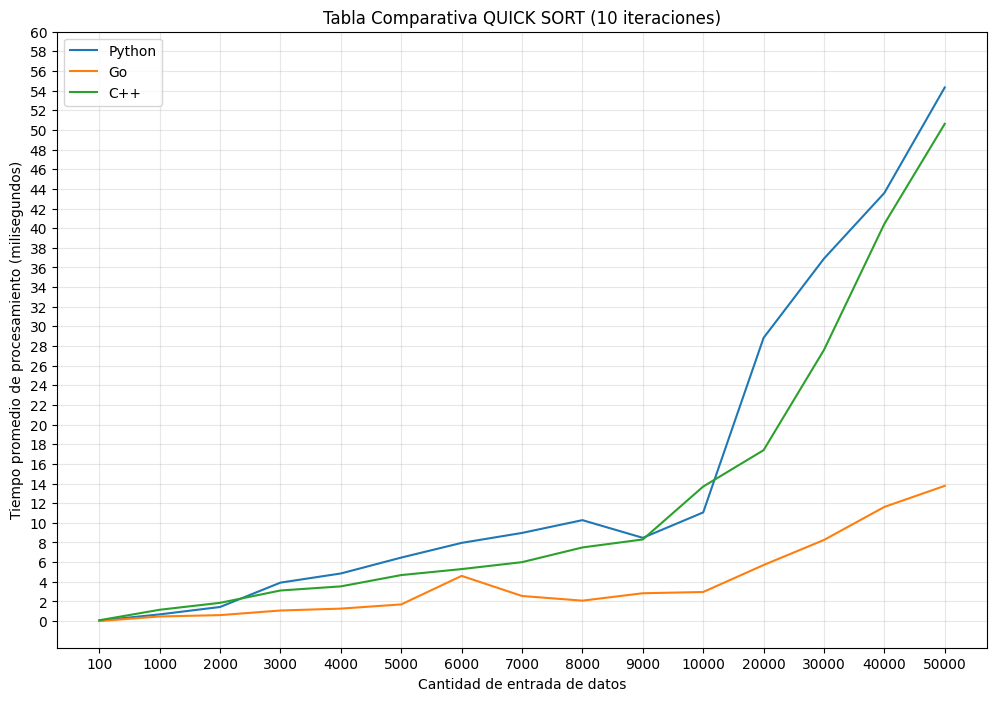
\includegraphics[width=0.95\textwidth]{GraphicQuickSort.png}
    \caption{\label{fig:bigOQuickSort}Gráfica comparativa Big-O del tiempo promedio de Ejecución Quick Sort}
    \end{figure}

% *****************************************************************

\section{CONCLUSIONES}
\begin{enumerate}
  \item xxxxxxxxxxxxxxxxxxxxxxxxxxxxxxxxxxxxxxxxxxxxxxxxxxxxxxxxxxxxxx
  \item xxxxxxxxxxxxxxxxxxxxxxxxxxxxxxxxxxxxxxxxxxxxxxxxxxxxxxxxxxxxxx
  \item xxxxxxxxxxxxxxxxxxxxxxxxxxxxxxxxxxxxxxxxxxxxxxxxxxxxxxxxxxxxxx
  \item xxxxxxxxxxxxxxxxxxxxxxxxxxxxxxxxxxxxxxxxxxxxxxxxxxxxxxxxxxxxxx
  \item xxxxxxxxxxxxxxxxxxxxxxxxxxxxxxxxxxxxxxxxxxxxxxxxxxxxxxxxxxxxxx

\end{enumerate}
Es importante tener en cuenta que los resultados de tiempo de ejecución pueden variar según el hardware y el entorno de ejecución utilizado para las pruebas. Se recomienda realizar pruebas adicionales y comparaciones en un contexto específico antes de tomar decisiones finales sobre qué algoritmo y lenguaje de programación utilizar en un proyecto real.


\begin{thebibliography}{widest entry} 
  \bibitem[1]{} Mamber, U. Introduction to Algorithms. A Creative Approach
  \bibitem[2]{} Cormen, Thomas; Leiserson, Charles; Rivest, Ronald; Stein, Clifford (2009). Introduction to Algorithms (Third ed.)
  \bibitem[3]{} Cormen, Thomas; Leiserson, Charles; Rivest, Ronald; Stein, Clifford (2009). Introduction to Algorithms (Third ed.)
  \bibitem[4]{} Astrachan, Owen (2003).
  \bibitem[5]{} Knuth, Donald (1998). "Section 5.2.4: Sorting by Merging". Sorting and Searching. The Art of Computer Programming
  \bibitem[6]{} ITIS IS04: Capítulo 10. Introducción al Análisis de Algoritmos
 \end{thebibliography}

\end{document}